% Beamer presentation
\documentclass[11pt,aspectratio=43,ignorenonframetext,t]{beamer}

% Presentation settings
\mode<presentation>{
  \usetheme[framenumber,titleframestart=1]{UoM_alex}
  \usefonttheme{professionalfonts} % using non standard fonts for beamer
  \usefonttheme{serif}
  \usepackage{fontspec}
  \setmainfont[Ligatures=TeX]{Arial}
}

% Handout settings
\mode<article>{
  \usepackage{fullpage}
  \usepackage{fontspec}
  \setmainfont[Ligatures=TeX]{Arial}
  \setlength{\parskip}{1.5\baselineskip} % correct beamer line spacings
  \setlength{\parindent}{0cm}
  \usepackage{enumitem}
  \setlist[itemize]{topsep=0pt}
}

 % Packages
\usepackage{graphicx}
\graphicspath{{./images/png}} % generic graphics path; overridden if necessary
\usepackage{amsmath}
\allowdisplaybreaks[1] % allow eqnarrays to break across pages
\usepackage{amssymb} 
\usepackage[HTML]{xcolor}
\definecolor{uomlinkblue}{HTML}{0071BC}
\usepackage{hyperref}
\hypersetup{
  colorlinks=true,
  linkcolor=uomlinkblue,
  filecolor=uomlinkblue,      
  urlcolor=uomlinkblue,
  pdflang={en-GB},
}
\usepackage[document]{ragged2e} % left aligned text for accessibility
\usepackage{tikz}
\usetikzlibrary{positioning, arrows, arrows.meta}
\usepackage{unicode-math} % unicode maths for accessibility
\usepackage{pdfcomment}   % for alt text for accessibility
\usepackage{rotating}     % allow portrait figures and tables
\usepackage{subfigure}    % allow matrices of figures
\usepackage{float}        % allows H option on floats to force here placement
\usepackage{multirow}     % allows merging of rows in tables
\usepackage{tabularx}     % allows fixed width tables
\usepackage{ctable}       % modifies \hline for use in table
\usepackage{bm}           % allow bold fonts in equations
\usepackage{pgf}          % allow graphics manipulation
\usepackage{etoolbox}
  
% Custom commands
\newcolumntype{Z}{>{\centering\arraybackslash}X}  % tabularx centered columns 

\makeatletter
  \DeclareRobustCommand{\em}
  {
    \@nomath\em
    \if b
      \expandafter\@car\f@series\@nil \normalfont
    \else
      \bfseries
    \fi
  }
\makeatother

\makeatletter
  \preto{\@verbatim}{\topsep=0pt \partopsep=0pt}
\makeatother

\def\checkmark{
  \tikz\fill[scale=0.4](0,.35) -- (.25,0) -- (1,.7) -- (.25,.15) -- cycle;
}

% Counters
\newcounter{example_number} % keep track of the example questions

% Frontmatter
\newcommand{\cmclecture}[1]{
  \title{Combinatorial Mesh Calculus (CMC): Lecture #1}
}
\author{
  Lectured by:
  \href{https://scholar.google.com/citations?user=x4R-snQAAAAJ&hl=en}
  {Dr. Kiprian Berbatov}$^1$\\
  \smallskip
  Lecture Notes Compiled by:
  \href{https://scholar.google.com/citations?user=CoIpITkAAAAJ&hl=en}
  {Muhammad Azeem}$^1$\\
  \smallskip
  Under the supervision of:
  \href{https://scholar.google.co.uk/citations?user=3nWJe5wAAAAJ&hl=en}
  {Prof. Andrey P. Jivkov}$^1$\\
  \smallskip
  {\tiny $^1$Department of Mechanical and Aerospace Engineering,
    The University of Manchester, Oxford Road, Manchester M13 9PL, UK}
}

% Special frames
\newcommand{\cmctitleframe}{
  \titlepage
  \begin{tikzpicture}[remember picture,overlay]
    \node[anchor=south east] at (current page.south east) {
      \href{https://youtube.com/@kipi.berbatov}{
        \includegraphics[width=1.5cm]{youtube-icon.png}
      }
    };
  \end{tikzpicture}
}
\newcommand{\cmcendframe}{
  \begin{figure}
    \centering
    \includegraphics[width=0.85\linewidth]{Thanks.png}
  \end{figure}
}

\cmclecture{14}
\date{05 November 2025}

\begin{document}

%========================= TITLE =========================
\begin{frame}
  \cmctitleframe
\end{frame}

\begin{frame}{$p$–Cells}
\begin{block}{Definition (CRWU context implicit for smoothness)}
Let $p\in\mathbb{N}$ and $X$ be a set.
\begin{itemize}
\item If $p=0$, then $X$ is a single point: a \emph{$0$–cell}.
\item If $p>0$, then $X$ is \emph{diffeomorphic} to an open $p$–ball (open interval, disk, ball): a \emph{$p$–cell}.
\end{itemize}
\end{block}

\begin{center}
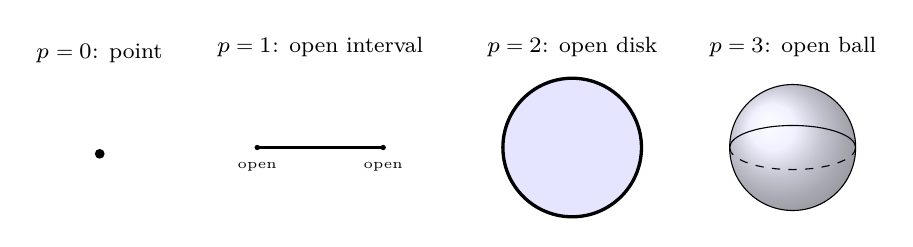
\begin{tikzpicture}[scale=0.8]
% p=0
\begin{scope}[xshift=-5.5cm,yshift=-0.1cm]
\node at (0,1.6) {\footnotesize $p=0$: point};
\fill (0,0) circle (2.2pt);
\end{scope}

% p=1 open interval
\begin{scope}[xshift=-2.0cm]
\node at (0,1.6) {\footnotesize $p=1$: open interval};
\draw[very thick] (-1,0)--(1,0);
\fill (-1,0) circle (1.2pt); \fill (1,0) circle (1.2pt);
\node at (-1,-0.3) {\tiny open};
\node at (1,-0.3) {\tiny open};
\end{scope}

% p=2 open disk
\begin{scope}[xshift=2.0cm]
\node at (0,1.6) {\footnotesize $p=2$: open disk};
\fill[blue!10] (0,0) circle (1.1);
\draw[very thick] (0,0) circle (1.1);
\end{scope}

% p=3 open ball (ghosted)
\begin{scope}[xshift=5.5cm]
\node at (0,1.6) {\footnotesize $p=3$: open ball};
\shade[ball color=blue!12,opacity=0.6] (0,0) circle (1.0);
\draw (0,0) circle (1.0);
\draw[dashed] (-1,0) arc (180:360:1 and 0.35);
\draw (-1,0) arc (180:0:1 and 0.35);
\end{scope}
\end{tikzpicture}
\end{center}
\end{frame}

%===========================

\begin{frame}{Regular Cell Complex}
\begin{block}{Definition}
Let $D\in\mathbb{N}$, $X$ a smooth $D$–manifold, and $\,\mathcal{M}\subseteq\mathcal{P}(X)$ a set of cells in $X$.
We say $\mathcal{M}$ is a \emph{regular cell complex} if:
\begin{itemize}
\item[(1)] For any $a,b\in\mathcal{M}$ with $a\neq b$, either $a\cap b=\varnothing$ or $\,a\cap b$ is a union of cells of strictly lower dimension.
\item[(2)] For any $a\in\mathcal{M}$, its closure in $X$ satisfies
\begin{align*}
\operatorname{cl}(a)
=\bigcup\{\,b\in\mathcal{M}\mid b\subseteq a\,\}.
\end{align*}
\end{itemize}
\end{block}
\end{frame}


\begin{frame}{Example}
    \begin{center}
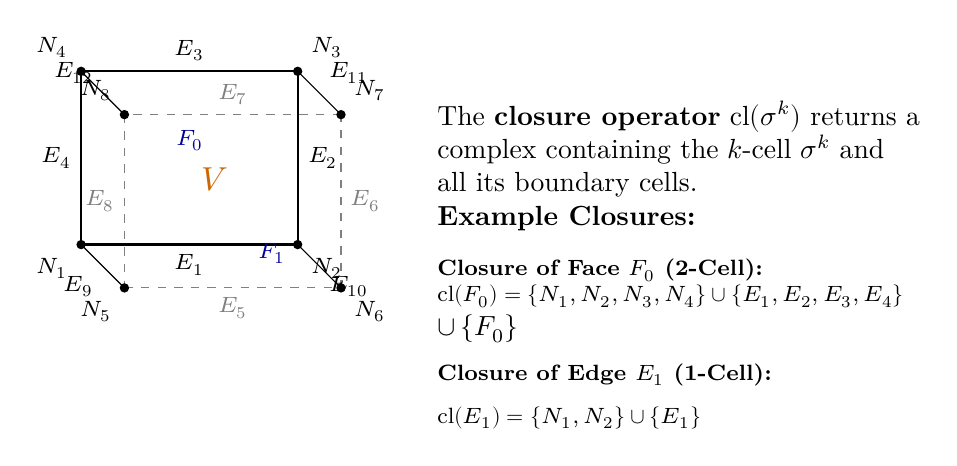
\begin{tikzpicture}[scale=1.1, dot/.style={fill, circle, inner sep=1.2pt}]

% --- 3D-like Cube Complex ---
\begin{scope}[xshift=-3.5cm]

    % Define coordinates for vertices (Nodes)
    \coordinate (N1) at (0,0);      % Front-Bottom-Left (FBL)
    \coordinate (N2) at (2.5,0);    % Front-Bottom-Right (FBR)
    \coordinate (N3) at (2.5,2);    % Front-Top-Right (FTR)
    \coordinate (N4) at (0,2);      % Front-Top-Left (FTL)

    \coordinate (N5) at (0.5,-0.5); % Back-Bottom-Left (BBL)
    \coordinate (N6) at (3.0,-0.5); % Back-Bottom-Right (BBR)
    \coordinate (N7) at (3.0,1.5);  % Back-Top-Right (BTR)
    \coordinate (N8) at (0.5,1.5);  % Back-Top-Left (BTL)

    % --- Edges (E_i) ---

    % Edges of the Back Face (F1) - Dotted lines for obscured view
    \draw[dashed, gray] (N5) -- (N6) node[midway, below] {\footnotesize $E_5$};
    \draw[dashed, gray] (N6) -- (N7) node[midway, right] {\footnotesize $E_6$};
    \draw[dashed, gray] (N7) -- (N8) node[midway, above] {\footnotesize $E_7$};
    \draw[dashed, gray] (N8) -- (N5) node[midway, left] {\footnotesize $E_8$};

    % Edges of the Front Face (F0)
    \draw[thick, black] (N1) -- (N2) node[midway, below] {\footnotesize $E_1$};
    \draw[thick, black] (N2) -- (N3) node[midway, right] {\footnotesize $E_2$};
    \draw[thick, black] (N3) -- (N4) node[midway, above] {\footnotesize $E_3$};
    \draw[thick, black] (N4) -- (N1) node[midway, left] {\footnotesize $E_4$};

    % Connecting Edges
    \draw[black] (N1) -- (N5) node[midway, below left] {\footnotesize $E_9$};
    \draw[black] (N2) -- (N6) node[midway, below right] {\footnotesize $E_{10}$};
    \draw[black] (N3) -- (N7) node[midway, above right] {\footnotesize $E_{11}$};
    \draw[black] (N4) -- (N8) node[midway, above left] {\footnotesize $E_{12}$};

    % --- Faces (F_i) & Volume (V) ---

    % Volume Label (V)
    \node[orange!80!black] at (1.5, 0.75) {\large $V$};

    % Face F0 Label (Front)
    \node[blue!60!black] at (1.25, 1.2) {\footnotesize $F_0$};

    % Face F1 Label (Back) - Slightly offset for clarity
    \node[blue!60!black] at (2.2, -0.1) {\footnotesize $F_1$};

    % --- Vertices (N_i) ---

    % Draw and Label Vertices (Nodes)
    \node[dot, label={below left:\footnotesize $N_1$}] at (N1) {};
    \node[dot, label={below right:\footnotesize $N_2$}] at (N2) {};
    \node[dot, label={above right:\footnotesize $N_3$}] at (N3) {};
    \node[dot, label={above left:\footnotesize $N_4$}] at (N4) {};

    \node[dot, label={below left:\footnotesize $N_5$}] at (N5) {};
    \node[dot, label={below right:\footnotesize $N_6$}] at (N6) {};
    \node[dot, label={above right:\footnotesize $N_7$}] at (N7) {};
    \node[dot, label={above left:\footnotesize $N_8$}] at (N8) {};

\end{scope}

% --- Closure Examples Text ---
\begin{scope}[xshift = 0.5cm, yshift=0.5cm]
\node[align=left, anchor=west] at (0,1.2) {
    \textbf{}
};
\node[align=left, anchor=west] at (0,0.6) {
    The \textbf{closure operator} $\operatorname{cl}(\sigma^k)$ returns a\\ complex containing the $k$-cell $\sigma^k$ and\\ all its boundary cells.
};

\node[align=left, anchor=west] at (0,-0.2) {
    \textbf{Example Closures:}
};

% Example for Face F0 (Front Face)
\node[align=left, anchor=west] at (0,-0.8) {\footnotesize
    \textbf{Closure of Face $F_0$ (2-Cell):}
};
\node[align=left, anchor=west] at (0,-1.3) {\footnotesize
    $\operatorname{cl}(F_0) = \left\{ N_1, N_2, N_3, N_4 \right\} \cup \left\{ E_1, E_2, E_3, E_4 \right\}$ \\$\cup \left\{ F_0 \right\}
    $
};

% Example for Edge E1 (Bottom Front Edge)
\node[align=left, anchor=west] at (0,-2.0) {\footnotesize
    \textbf{Closure of Edge $E_1$ (1-Cell):}
};
\node[align=left, anchor=west] at (0,-2.5) {\footnotesize
    $\operatorname{cl}(E_1) = \left\{ N_1, N_2 \right\} \cup \left\{ E_1 \right\}$
};

\end{scope}
\end{tikzpicture}
\end{center}
\end{frame}
%===========================

\begin{frame}{Faces and Partial Order}
\begin{block}{Remark (Face relation)}
A regular cell complex $\mathcal{M}$ carries a partial order by inclusion: $a\subseteq b$.
We write $a\preccurlyeq b$ and say ``$a$ is a \emph{face} of $b$''.
\end{block}

\begin{block}{Hasse-type diagram (schematic)}
\begin{center}
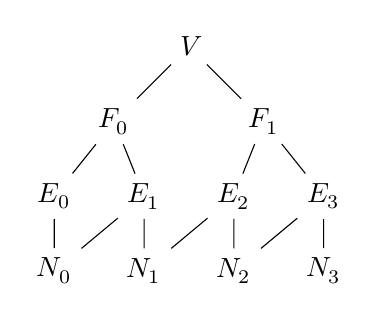
\begin{tikzpicture}[scale=0.95]
% top cell
\node (V) at (0,1.8) {$V$};
% faces
\node (F1) at (-1,0.8) {$F_0$};
\node (F2) at ( 1,0.8) {$F_1$};
% edges
\node (E0) at (-1.8,-0.2) {$E_0$};
\node (E1) at (-0.6,-0.2) {$E_1$};
\node (E2) at ( 0.6,-0.2) {$E_2$};
\node (E3) at ( 1.8,-0.2) {$E_3$};
% nodes
\node (N0) at (-1.8,-1.2) {$N_0$};
\node (N1) at (-0.6,-1.2) {$N_1$};
\node (N2) at ( 0.6,-1.2) {$N_2$};
\node (N3) at ( 1.8,-1.2) {$N_3$};

% relations
\draw (V)--(F1); \draw (V)--(F2);
\draw (F1)--(E0); \draw (F1)--(E1);
\draw (F2)--(E2); \draw (F2)--(E3);
\draw (E0)--(N0); \draw (E1)--(N0);
\draw (E1)--(N1); \draw (E2)--(N1);
\draw (E2)--(N2); \draw (E3)--(N2);
\draw (E3)--(N3);
\end{tikzpicture}
\end{center}
\end{block}
\end{frame}

%===========================

\begin{frame}{Combinatorial Mesh}

\begin{block}{Definition}
A partially ordered set $(\mathcal{M},\preccurlyeq)$ is a \emph{combinatorial mesh} if there exists a manifold $X$ and an embedding
$\varphi:\mathcal{M}\to \mathcal{P}(X)$ whose image is a regular cell complex in $X$.
\end{block}

\begin{block}{Relational data (example)}
\begin{align*}
&F_0\prec E_0,E_1,\\
&F_1\prec E_2,E_3,\\
&E_0\prec N_0,\ \ E_1\prec N_0,N_1,\\ &E_2\prec N_1,N_2,\ \ E_3\prec N_2.
\end{align*}
\end{block}
\end{frame}

\begin{frame}{Example}
\vspace{-0.9cm}
    \begin{center}
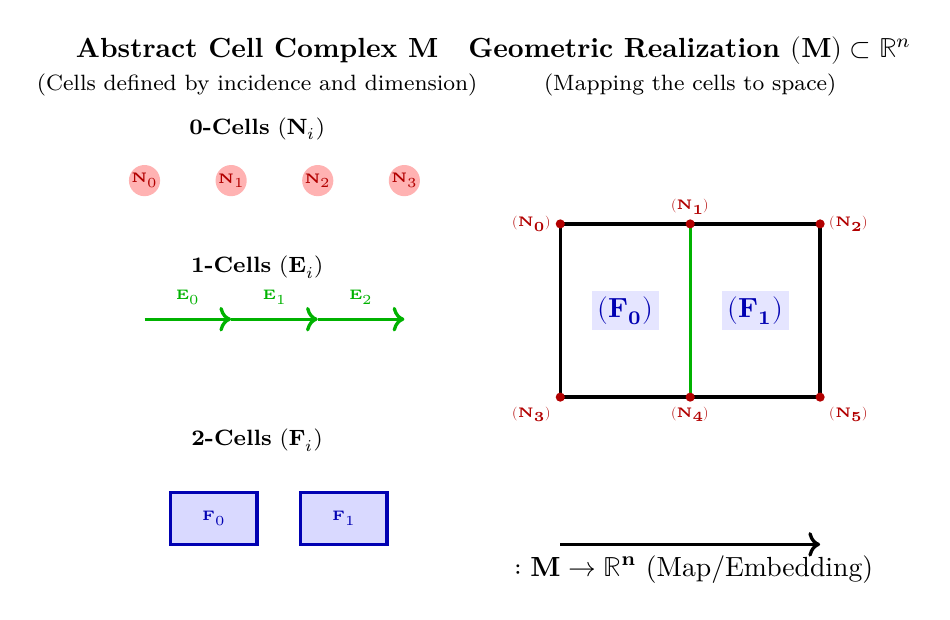
\begin{tikzpicture}[scale=1.1, dot/.style={fill, circle, inner sep=1.2pt}]

% --- LEFT SIDE: ABSTRACT CELL COMPLEX (K) ---
\begin{scope}[xshift=-4.5cm]
\node at (0, 2.5) {\textbf{Abstract Cell Complex $\mathbf{M}$}};
\node at (0, 2.1) {\footnotesize (Cells defined by incidence and dimension)};

% --- 0-cells (Vertices/Nodes) ---
\node at (0, 1.6) {\footnotesize \textbf{0-Cells} ($\mathbf{N}_i$)};
\fill[red!30] (-1.3, 1) circle (0.18cm); \node[red!70!black] at (-1.3, 1) {\tiny $\mathbf{N}_0$};
\fill[red!30] (-0.3, 1) circle (0.18cm); \node[red!70!black] at (-0.3, 1) {\tiny $\mathbf{N}_1$};
\fill[red!30] (0.7, 1) circle (0.18cm); \node[red!70!black] at (0.7, 1) {\tiny $\mathbf{N}_2$};
\fill[red!30] (1.7, 1) circle (0.18cm); \node[red!70!black] at (1.7, 1) {\tiny $\mathbf{N}_3$};

% --- 1-cells (Edges) ---
\node at (0, 0) {\footnotesize \textbf{1-Cells} ($\mathbf{E}_i$)};
\draw[green!70!black, very thick, ->] (-1.3, -0.6) -- (-0.3, -0.6); \node[green!70!black] at (-0.8, -0.35) {\tiny $\mathbf{E}_0$};
\draw[green!70!black, very thick, ->] (-0.3, -0.6) -- (0.7, -0.6); \node[green!70!black] at (0.2, -0.35) {\tiny $\mathbf{E}_1$};
\draw[green!70!black, very thick, ->] (0.7, -0.6) -- (1.7, -0.6); \node[green!70!black] at (1.2, -0.35) {\tiny $\mathbf{E}_2$};

% --- 2-cells (Faces/Patches) ---
\node at (0, -2.0) {\footnotesize \textbf{2-Cells} ($\mathbf{F}_i$)};
\fill[blue!15, draw=blue!70!black, very thick] (-1.0, -2.6) rectangle (0.0, -3.2); \node[blue!70!black] at (-0.5, -2.9) {\tiny $\mathbf{F}_0$};
\fill[blue!15, draw=blue!70!black, very thick] (0.5, -2.6) rectangle (1.5, -3.2); \node[blue!70!black] at (1.0, -2.9) {\tiny $\mathbf{F}_1$};
\end{scope}

\begin{scope}[xshift=0.5cm]
\node at (0, 2.5) {\textbf{Geometric Realization $\mathbf{\varphi(M)} \subset \mathbb{R}^n$}};
\node at (0, 2.1) {\footnotesize (Mapping the cells to space)};

\draw[very thick] (-1.5, 0.5) -- (1.5, 0.5); % Top Edge
\draw[very thick] (-1.5, -1.5) -- (1.5, -1.5); % Bottom Edge
\draw[very thick] (-1.5, 0.5) -- (-1.5, -1.5); % Left Edge
\draw[very thick, green!70!black] (0, 0.5) -- (0, -1.5); % Common Edge (E_1)
\draw[very thick] (1.5, 0.5) -- (1.5, -1.5); % Right Edge

\fill[red!70!black] (-1.5, 0.5) circle (1.5pt) node[left] {\tiny $\mathbf{\varphi(N_0)}$};
\fill[red!70!black] (0, 0.5) circle (1.5pt) node[above] {\tiny $\mathbf{\varphi(N_1)}$};
\fill[red!70!black] (1.5, 0.5) circle (1.5pt) node[right] {\tiny $\mathbf{\varphi(N_2)}$};
\fill[red!70!black] (-1.5, -1.5) circle (1.5pt) node[below left] {\tiny $\mathbf{\varphi(N_3)}$}; % New node for bottom left
\fill[red!70!black] (0, -1.5) circle (1.5pt) node[below] {\tiny $\mathbf{\varphi(N_4)}$};    % New node for bottom center
\fill[red!70!black] (1.5, -1.5) circle (1.5pt) node[below right] {\tiny $\mathbf{\varphi(N_5)}$}; % New node for bottom right

% --- Realized 2-cells (Faces) ---
\node[blue!70!black, fill=blue!10, inner sep=2pt] at (-0.75, -0.5) {$\mathbf{\varphi(F_0)}$};
\node[blue!70!black, fill=blue!10, inner sep=2pt] at (0.75, -0.5) {$\mathbf{\varphi(F_1)}$};

% --- Mapping text ---
\draw[->, very thick] (-1.5, -3.2) -- (1.5, -3.2) node[midway, below] {$\mathbf{\varphi: M \to \mathbb{R}^n}$ (Map/Embedding)};
\end{scope}
\end{tikzpicture}
\end{center}
\end{frame}

%===========================

\begin{frame}{Combinatorial Polytopes and Digon}
\begin{block}{Remark }
If $\mathcal{M}$ is a combinatorial mesh, the set of $p$–cells is $\mathcal{M}_p$.
If $D$ is the maximum dimension, then $\mathcal{M}=\bigcup_{p=0}^{D}\mathcal{M}_p$.
If there exists a single top $D$–cell containing all cells, the mesh is a \emph{combinatorial polytope}.
\end{block}

\begin{center}
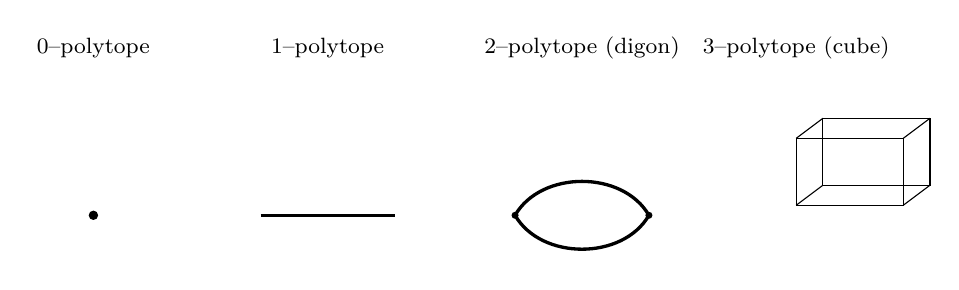
\begin{tikzpicture}[scale=0.85]
% 0-polytope: point
\begin{scope}[xshift=-5.5cm]
\node at (0,2.5) {\footnotesize 0–polytope};
\fill (0,0) circle (2pt);
\end{scope}

% 1-polytope: segment
\begin{scope}[xshift=-2.0cm]
\node at (0,2.5) {\footnotesize 1–polytope};
\draw[very thick] (-1,0)--(1,0);
\end{scope}

% 2-polytope: digon (two edges, two vertices)
\begin{scope}[xshift=1.8cm]
\node at (0,2.5) {\footnotesize 2–polytope (digon)};
\draw[very thick] (-1,0) to[out=60,in=120] (1,0);
\draw[very thick] (-1,0) to[out=-60,in=-120] (1,0);
\fill (-1,0) circle (1.5pt);\fill (1,0) circle (1.5pt);
\end{scope}

% 3-polytope: cube (wireframe)
\begin{scope}[xshift=5.0cm, yshift=0.15cm]
\node at (0, 2.35) {\footnotesize 3–polytope (cube)};
\draw (0,0) rectangle (1.6,1.0);
\draw (0.4,0.3) rectangle (2.0,1.3);
\draw (0,0)--(0.4,0.3);\draw (1.6,0)--(2.0,0.3);
\draw (1.6,1.0)--(2.0,1.3);\draw (0,1.0)--(0.4,1.3);
\end{scope}
\end{tikzpicture}
\end{center}
\end{frame}

%===========================

\begin{frame}{Diamond Property}
\begin{block}{Proposition}
Let $\mathcal{M}$ be a combinatorial mesh, $p\in\mathbb{N}$, $a\in\mathcal{M}_{p+2}$ and $c\in\mathcal{M}_p$ with $c\preccurlyeq a$.
Then there exist exactly two $(p+1)$–cells $\,b',b''\in\mathcal{M}_{p+1}$ such that
\vspace{-0.3cm}
\begin{align*}
c\preccurlyeq b',\quad c\preccurlyeq b'',\qquad b'\preccurlyeq a,\quad b''\preccurlyeq a.
\end{align*}
\end{block}

\begin{center}
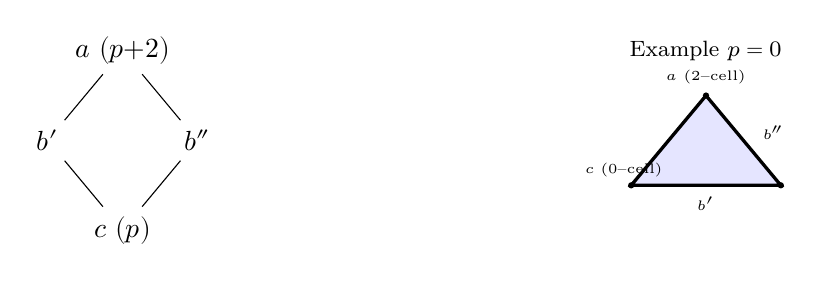
\begin{tikzpicture}[scale=0.95]
% Abstract diamond
\begin{scope}[xshift=-3.9cm]
\node (a) at (0,1.8) {$a\ (p{+}2)$};
\node (bp) at (-1,0.6) {$b'$};
\node (bq) at ( 1,0.6) {$b''$};
\node (c)  at (0,-0.6) {$c\ (p)$};
\draw (a)--(bp)--(c)--(bq)--(a);
\end{scope}

% Examples: p=0 (triangle)
\begin{scope}[xshift=3.9cm]
\node at (0,1.8) {\footnotesize Example $p=0$};
% triangle: a = filled triangle (2-cell), b' and b'' edges, c vertex
\coordinate (A) at (-1,0);
\coordinate (B) at (1,0);
\coordinate (C) at (0,1.2);
\fill[blue!10] (A)--(B)--(C)--cycle;
\draw[very thick] (A)--(B)--(C)--cycle;
\fill (A) circle (1.2pt);\fill (B) circle (1.2pt);\fill (C) circle (1.2pt);
\node at (0,1.45) {\tiny $a$ (2–cell)};
\node at (-1.1,0.2) {\tiny $c$ (0–cell)};
\node at (0,-0.25) {\tiny $b'$};
\node at (0.9,0.7) {\tiny $b''$};
\end{scope}
\end{tikzpicture}
\end{center}
\end{frame}

%===========================

\begin{frame}{Diamond Property: $p=1$ Example}
\begin{block}{Cube Slice}

\end{block}\begin{center}
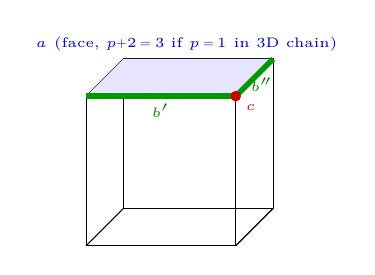
\begin{tikzpicture}[scale=0.95]
% cube wireframe
\draw (0,0) rectangle (2,2);
\draw (0.5,0.5) rectangle (2.5,2.5);
\draw (0,0)--(0.5,0.5);\draw (2,0)--(2.5,0.5);
\draw (2,2)--(2.5,2.5);\draw (0,2)--(0.5,2.5);

% take a = a square face (top front)
\fill[blue!10] (0.5,2.5) -- (2.5,2.5) -- (2,2) -- (0,2) -- cycle;
\node[blue!70!black] at (1.35,2.7) {\tiny $a$ (face, $p{+}2=3$ if $p=1$ in 3D chain)};

% two edges b', b''
\draw[line width=2pt,green!60!black] (0,2)--(2,2); \node[green!50!black] at (1.0,1.8) {\tiny $b'$};
\draw[line width=2pt,green!60!black] (2,2)--(2.5,2.5); \node[green!50!black] at (2.35,2.15) {\tiny $b''$};

% vertex c
\fill[red!80!black] (2,2) circle (2pt); \node[red!80!black] at (2.2,1.85) {\tiny $c$};

\end{tikzpicture}
\end{center}

\begin{block}{Interpretation}
For $p=1$ in 3D, let $a$ be a face, $c$ a vertex on $a$. Exactly two edges $b',b''$ on $a$ meet at $c$, forming the diamond.
\end{block}
\end{frame}

%===========================
%===========================
% ORIENTATIONS, CHAINS, BOUNDARY OPERATORS ON A COMBINATORIAL MESH
%===========================

%------------------------------------------------
\begin{frame}{Relative Orientations}
\vspace{-0.2cm}
\begin{block}{Theorem (Relative Orientation)}
Let $M$ be a combinatorial mesh (CM). Then there exist signs
$\epsilon(a,b)\in\{-1,1\}$, for any incident pair $(a,b)\in M_{p+1}\times M_p$ with $b\prec a$ (``$b$ is a face of $a$''), called the \emph{relative orientation}, such that for each diamond
\[
c\in M_p,\quad b',b''\in M_{p+1},\quad a\in M_{p+2},\qquad
c\preccurlyeq b',b''\preccurlyeq a,
\]
the following holds:
\vspace{-0.3cm}
\begin{align*}
\epsilon(a,b')\,\epsilon(b',c)\;=\;-\;\epsilon(a,b'')\,\epsilon(b'',c).
\end{align*}
Moreover, if an edge $E$ has endpoints (nodes) $N',N''$, then
\vspace{-0.3cm}
\begin{align*}
\epsilon(E,N') \;=\; -\,\epsilon(E,N'').
\end{align*}
\end{block}
\end{frame}

\begin{frame}{Example}
    \begin{block}{}
        \begin{center}
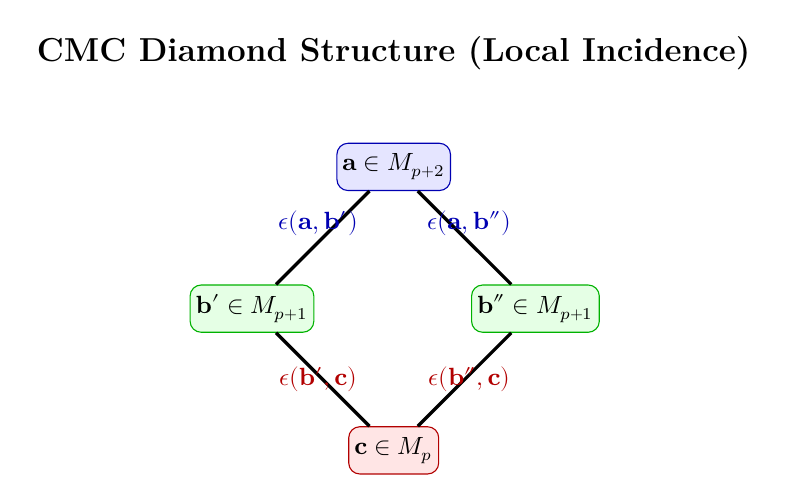
\begin{tikzpicture}[scale=1.2, every node/.style={font=\small}]

% --- Vertices (Nodes) and Cell Labels ---
% p+2 Cell (Highest Dimension, represented by 'a') - Blue
\node[fill=blue!10, draw=blue!70!black, rounded corners, minimum size=6mm, inner sep=2pt] (a) at (0, 2.0) {$\mathbf{a} \in M_{p+2}$};

% p+1 Cells (Intermediate Dimension, represented by 'b' and 'b'') - Green
\node[fill=green!10, draw=green!70!black, rounded corners, minimum size=6mm, inner sep=2pt] (bp) at (-1.5, 0.5) {$\mathbf{b'} \in M_{p+1}$};
\node[fill=green!10, draw=green!70!black, rounded corners, minimum size=6mm, inner sep=2pt] (bq) at ( 1.5, 0.5) {$\mathbf{b''} \in M_{p+1}$};

% p Cell (Lowest Dimension, represented by 'c') - Red
\node[fill=red!10, draw=red!70!black, rounded corners, minimum size=6mm, inner sep=2pt] (c) at (0, -1.0) {$\mathbf{c} \in M_{p}$};

% --- Incidence Edges (Lines) ---
% Using thick black lines to represent the boundary/incidence
\draw[very thick] (a) -- (bp);
\draw[very thick] (a) -- (bq);
\draw[very thick] (bp) -- (c);
\draw[very thick] (bq) -- (c);

% --- Incidence Number (Signs) Labels ---
% Labels are placed next to the edges they define, emphasizing the local sign structure

% Signs for (p+2) and (p+1) cell incidence
\node[blue!70!black] at (-0.8, 1.4) {$\epsilon(\mathbf{a},\mathbf{b'})$};
\node[blue!70!black] at ( 0.8, 1.4) {$\epsilon(\mathbf{a},\mathbf{b''})$};

% Signs for (p+1) and (p) cell incidence
\node[red!70!black] at (-0.8, -0.25) {$\epsilon(\mathbf{b'},\mathbf{c})$};
\node[red!70!black] at ( 0.8, -0.25) {$\epsilon(\mathbf{b''},\mathbf{c})$};

% --- Title/Context ---
\node[font=\large\bfseries] at (0, 3.2) {CMC Diamond Structure (Local Incidence)};

\end{tikzpicture}
\end{center}
    \end{block}
\end{frame}
%------------------------------------------------
\begin{frame}{Chains and the Boundary Operator}
\begin{block}{Definition}
Let $M$ be a combinatorial $D$–dimensional mesh. For $p\in\{0,1,\dots,D\}$ let
\[
C_p M:=\mathrm{Free}_{\mathbb{R}}(M_p)
=\Big\{\sum_{i=1}^{n}\lambda_i a_i\ \Big|\ \lambda_i\in\mathbb{R},\,a_i\in M_p\Big\}.
\]
The space of all chains is $C_{\bullet}M=\bigoplus_{p=0}^{D} C_p M$.

Given a choice of relative orientations $\epsilon$, define
\vspace{-0.3cm}
\begin{align*}
\partial_p: C_p M \longrightarrow C_{p-1} M,\qquad
\partial_p a \;=\;\sum_{\substack{b\prec a\\ b\in M_{p-1}}}\epsilon(a,b)\,b,
\quad a\in M_p.
\end{align*}
If we fix the standard bases (cells ordered, with signs by $\epsilon$), the matrix of $\partial_p$
is denoted $\overline{\partial}_p$.
\end{block}
\end{frame}

%------------------------------------------------
\begin{frame}{Example Mesh}
\vspace{-0.3cm}
\begin{block}{Triangular with a Diagonal}
\begin{center}
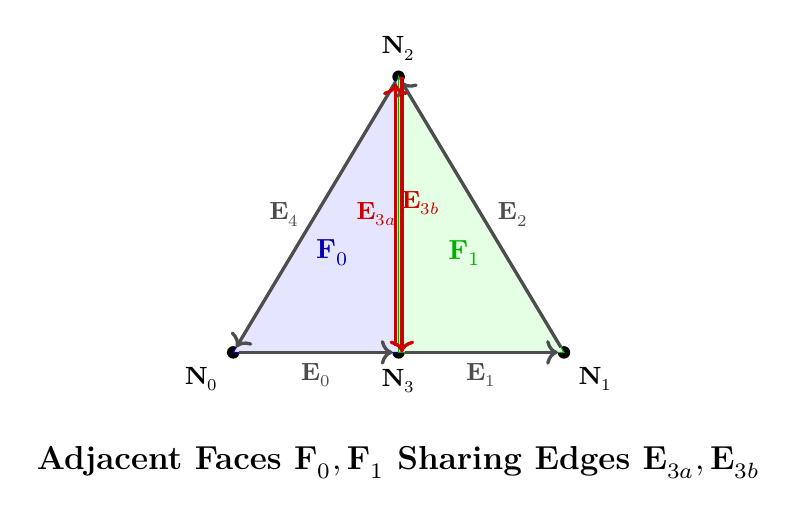
\begin{tikzpicture}[scale=1.4, dot/.style={fill, circle, inner sep=1.6pt}]

\coordinate (N0) at (0,0);
\coordinate (N1) at (3.0,0);
\coordinate (N2) at (1.5, 2.5);
\coordinate (N3) at (1.5, 0);

\node[dot, label={below left:\small $\mathbf{N}_0$}] at (N0) {};
\node[dot, label={below right:\small $\mathbf{N}_1$}] at (N1) {};
\node[dot, label={above:\small $\mathbf{N}_2$}] at (N2) {};
\node[dot, label={below:\small $\mathbf{N}_3$}] at (N3) {};


\fill[blue!10, draw=blue!70!black, thin] (N0) -- (N3) -- (N2) -- cycle;
\node[blue!70!black] at (0.9, 0.9) {$\mathbf{F}_0$};

\fill[green!10, draw=green!70!black, thin] (N3) -- (N1) -- (N2) -- cycle;
\node[green!70!black] at (2.1, 0.9) {$\mathbf{F}_1$};

\def\arrowshorten{2.2pt}
\draw[very thick, black!70, ->, shorten >= \arrowshorten, shorten <= \arrowshorten] (N0) -- (N3) node[midway, below] {\small $\mathbf{E}_0$};

\draw[very thick, black!70, ->, shorten >= \arrowshorten, shorten <= \arrowshorten] (N3) -- (N1) node[midway, below] {\small $\mathbf{E}_1$};

\draw[very thick, black!70, ->, shorten >= \arrowshorten, shorten <= \arrowshorten] (N1) -- (N2) node[pos=0.5, right, xshift=2pt] {\small $\mathbf{E}_2$};

\draw[very thick, black!70, ->, shorten >= \arrowshorten, shorten <= \arrowshorten] (N2) -- (N0) node[pos=0.5, left, xshift=-2pt] {\small $\mathbf{E}_4$};

\coordinate (N3_offset_left)  at (1.47, 0.03);
\coordinate (N2_offset_left)  at (1.47, 2.47);
\coordinate (N3_offset_right) at (1.53, -0.03);
\coordinate (N2_offset_right) at (1.53, 2.53);


\draw[very thick, red!80!black, ->, shorten >= 1.2pt, shorten <= 1.2pt] (N3_offset_left) -- (N2_offset_left);
\node[red!80!black] at (1.3, 1.25) {\small $\mathbf{E}_{3a}$}; %

\draw[very thick, red!80!black, ->, shorten >= 1.2pt, shorten <= 1.2pt] (N2_offset_right) -- (N3_offset_right);
\node[red!80!black] at (1.7, 1.35) {\small $\mathbf{E}_{3b}$}; %

\node[font=\large\bfseries] at (1.5, -1.0) {Adjacent Faces $\mathbf{F}_0, \mathbf{F}_1$ Sharing Edges $\mathbf{E}_{3a}, \mathbf{E}_{3b}$};
\end{tikzpicture}
\end{center}
\end{block}
\end{frame}


\begin{frame}{Example}
\begin{block}{Chosen Orientations}
Edges:
\vspace{-0.4cm}
\begin{align*}
    &E_0: N_0\!\to\!N_3,\\
    &E_1: N_3\!\to\!N_1,\\
    &E_2: N_1\!\to\!N_2,\\
    &E_{3a}: N_3\!\to\!N_2,\\
    &E_{3b}: N_2\!\to\!N_3,\\
    &E_4: N_2\!\to\!N_0.
\end{align*}

Faces (counterclockwise):
\vspace{-0.2cm}
\begin{align*}
    &F_0: (N_0\!\to\!N_3\!\to\!N_2\!\to\!N_0),\\
    &F_1: (N_3\!\to\!N_1\!\to\!N_2\!\to\!N_3).
\end{align*}
\end{block}

\end{frame}

%------------------------------------------------
\begin{frame}{Boundary on Edges and Faces}
\begin{block}{Edge Boundaries ($\partial_1: C_1\to C_0$)}
\vspace{-0.3cm}
\begin{align*}
\partial_1(E_0) &= N_3 - N_0, &
\partial_1(E_1) &= N_1 - N_3, &
\partial_1(E_2) &= N_2 - N_1,\\
\partial_1(E_{3a}) &= N_2 - N_3, &
\partial_1(E_{3b}) &= N_3 - N_2, &
\partial_1(E_4) &= N_0 - N_2.
\end{align*}
\end{block}

\begin{block}{Face Boundaries ($\partial_2: C_2\to C_1$)}
\vspace{-0.3cm}
\begin{align*}
\partial_2(F_0) &= E_0 + E_{3a} + E_4,\\
\partial_2(F_1) &= E_1 + E_2 + E_{3b}.
\end{align*}
\end{block}
\end{frame}


\begin{frame}{Boundary on Edges and Faces}
\vspace{-0.3cm}
\begin{block}{Matrices in the Ordered Bases}
Let rows/cols be ordered as indicated under each matrix.
\vspace{-0.3cm}
\begin{align*}
\overline{\partial}_1
&=\big(\partial_1\big)_{E}^{N}
=
\begin{array}{c}
\\[-0.2cm]
\scriptstyle N_0\\[-0.05cm]
\scriptstyle N_1\\[-0.05cm]
\scriptstyle N_2\\[-0.05cm]
\scriptstyle N_3
\end{array}
\left[
\begin{array}{cccccc}
\scriptstyle E_0 & \scriptstyle E_1 & \scriptstyle E_2 & \scriptstyle E_{3a} & \scriptstyle E_{3b} & \scriptstyle E_4\\ \hline
-1 &  0 &  0 &  0 &  0 &  1\\
 0 &  1 & -1 &  0 &  0 &  0\\
 0 &  0 &  1 &  1 & -1 & -1\\
 1 & -1 &  0 & -1 &  1 &  0
\end{array}
\right],\\[6pt]
\overline{\partial}_2
&=\big(\partial_2\big)_{F}^{E}
=
\begin{array}{c}
\\[-0.2cm]
\scriptstyle E_0\\[-0.05cm]
\scriptstyle E_1\\[-0.05cm]
\scriptstyle E_2\\[-0.05cm]
\scriptstyle E_{3a}\\[-0.05cm]
\scriptstyle E_{3b}\\[-0.05cm]
\scriptstyle E_4
\end{array}
\left[
\begin{array}{cc}
\scriptstyle F_0 & \scriptstyle F_1\\ \hline
 1 &  0\\
 0 &  1\\
 0 &  1\\
 1 &  0\\
 0 &  1\\
 1 &  0
\end{array}
\right].
\end{align*}
\vspace{-0.3cm}
\end{block}
\end{frame}



%------------------------------------------------
\begin{frame}{Nilpotency of the Boundary: \(\partial\circ\partial=0\)}
\begin{block}{Theorem (Chain Complex Property)}
For any combinatorial mesh $M$ and any $p\in\mathbb{N}$,
\vspace{-0.3cm}
\begin{align*}
\partial_{p}\circ \partial_{p+1} = 0
\;:\; C_{p+1}M \longrightarrow C_{p-1}M,
\end{align*}
equivalently, in matrix form,
\vspace{-0.3cm}
\begin{align*}
\overline{\partial}_{p}\,\overline{\partial}_{p+1}=\overline{0}
\in \mathbb{R}^{\,|M_{p-1}|\times |M_{p+1}|}.
\end{align*}
\end{block}
\end{frame}


\begin{frame}{Example}
\vspace{-0.3cm}
    \begin{block}{Verification in the Example}
Using the previous matrices,
\vspace{-0.3cm}
\begin{align*}
\overline{\partial}_1\,\overline{\partial}_2
&=
\begin{bmatrix}
-1 & 0 & 0 & 0 & 0 & 1\\
 0 & 1 & -1 & 0 & 0 & 0\\
 0 & 0 & 1 & 1 & -1 & -1\\
 1 & -1 & 0 & -1 & 1 & 0
\end{bmatrix}
\begin{bmatrix}
 1 &  0\\
 0 &  1\\
 0 &  1\\
 1 &  0\\
 0 &  1\\
 1 &  0
\end{bmatrix}
=
\begin{bmatrix}
0 & 0\\
0 & 0\\
0 & 0\\
0 & 0
\end{bmatrix}.
\end{align*}


\vspace{-0.8cm}
\begin{center}
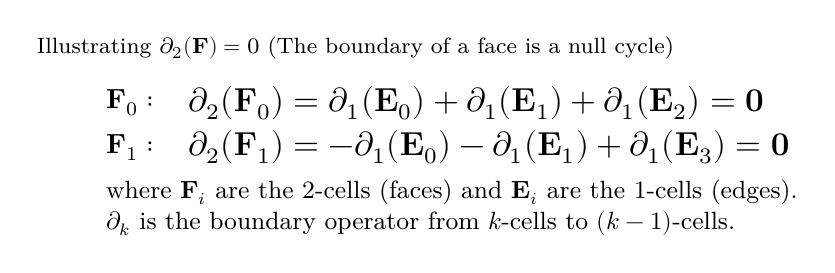
\begin{tikzpicture}[scale=0.7]
\node[font=\footnotesize] at (+1.2, 1.4) {Illustrating $\partial_2(\mathbf{F}) = 0$ (The boundary of a face is a null cycle)};

\node[anchor=west] at (-3.5, 0.4) {$\mathbf{F}_0:$};
\node[anchor=west, font=\large] at (-2.0, 0.4) {
    $\partial_2(\mathbf{F}_0) = \partial_1(\mathbf{E}_0) + \partial_1(\mathbf{E}_1) + \partial_1(\mathbf{E}_2) = \mathbf{0}$
};

\node[anchor=west] at (-3.5, -0.4) {$\mathbf{F}_1:$};
\node[anchor=west, font=\large] at (-2.0, -0.4) {
    $\partial_2(\mathbf{F}_1) = -\partial_1(\mathbf{E}_0) - \partial_1(\mathbf{E}_1) + \partial_1(\mathbf{E}_3) = \mathbf{0}$
};

\node[anchor=west, align=left, font=\small] at (-3.5, -1.5) {
    where $\mathbf{F}_i$ are the 2-cells (faces) and $\mathbf{E}_i$ are the 1-cells (edges). \\
    $\partial_k$ is the boundary operator from $k$-cells to $(k-1)$-cells.
};

\end{tikzpicture}
\end{center}
\end{block}
\end{frame}



%===========================================================
% CHAINS, COCHAINS, COBoundary, DE RHAM, AND TRACE (DISCRETE vs SMOOTH)
%===========================================================

%---------------------------
\begin{frame}{Remark}
\begin{block}{Boundary Operator and Chain Complex}
For a combinatorial $D$–mesh $M$, the chain spaces $(C_pM)_{p=0}^D$ with boundary maps
\[
C_D M \xrightarrow{\;\partial_D\;} C_{D-1} M \xrightarrow{\;\partial_{D-1}\;} \cdots
\xrightarrow{\;\partial_2\;} C_1 M \xrightarrow{\;\partial_1\;} C_0 M
\]
form a chain complex.
\vspace{-0.3cm}
\begin{align*}
\text{Chain complex property:}\qquad
\partial_{p}\circ \partial_{p+1}=0,\quad \forall\,p\in\{0,\dots,D-1\}.
\end{align*}
\end{block}

\begin{center}
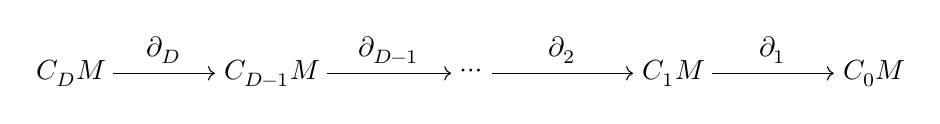
\begin{tikzpicture}[scale=0.85]
\node (CD)   at (0,0) {$C_D M$};
\node (CDm1) at (3,0) {$C_{D-1} M$};
\node (dots) at (6,0) {$\cdots$};
\node (C1)   at (9,0) {$C_1 M$};
\node (C0)   at (12,0){$C_0 M$};

\draw[->] (CD) -- node[above] {$\partial_D$}   (CDm1);
\draw[->] (CDm1) -- node[above] {$\partial_{D-1}$} (dots);
\draw[->] (dots) -- node[above] {$\partial_{2}$} (C1);
\draw[->] (C1) -- node[above] {$\partial_{1}$} (C0);
\end{tikzpicture}
\end{center}
\end{frame}

%---------------------------
\begin{frame}{Cochains and Coboundary}
\vspace{-0.2cm}
\begin{block}{Definition (Cochains and Coboundary)}
Let $(M,\epsilon)$ be a $D$–dimensional CM with a fixed system of relative orientations.
For $p\in\{0,\dots,D\}$, the space of $p$–cochains is the $\mathbb{R}$–linear dual
\[
C^p M := (C_p M)^*,\qquad C^\bullet M:=\bigoplus_{p=0}^D C^p M.
\]
Choose dual bases concretely:
\[
\begin{aligned}
&p=0:\ (N^0,N^1,\dots)\ \text{dual to}\ (N_0,N_1,\dots),\\
&p=1:\ (E^0,E^1,\dots)\ \text{dual to}\ (E_0,E_1,\dots),\\
&p=2:\ (F^0,F^1,\dots)\ \text{dual to}\ (F_0,F_1,\dots),\\
&p=3:\ (V^0,V^1,\dots)\ \text{dual to}\ (V_0,V_1,\dots).
\end{aligned}
\]
\end{block}
\end{frame}

\begin{frame}{Cochains and Coboundary}
\begin{block}{Definition (Cochains and Coboundary)}
The coboundary operators $\delta_p:C^pM\to C^{p+1}M$ are the duals of $\partial_{p+1}$:
\vspace{-0.3cm}
\begin{align*}
\delta_p \sigma \;=\; \sigma\circ \partial_{p+1}\in C^{p+1}M,\qquad
\overline{\delta}_p \;=\; \overline{\partial}_{p+1}^{\,\mathsf{T}}.
\end{align*}
\end{block}

\begin{block}{Cochain Complex Property}
\vspace{-0.3cm}
\begin{align*}
\delta_{p+1}\circ \delta_p \;=\; 0,\qquad \forall\,p\in\{0,\dots,D-1\}.
\end{align*}
\end{block}
\vspace{-0.3cm}
\begin{center}
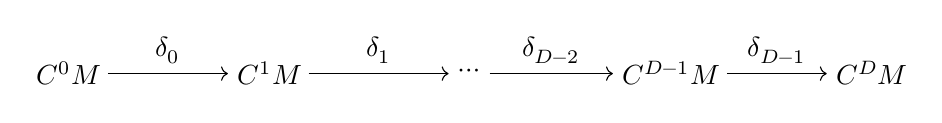
\begin{tikzpicture}[scale=0.85]
\node (C0)   at (0,0) {$C^0 M$};
\node (C1)   at (3,0) {$C^1 M$};
\node (dots) at (6,0) {$\cdots$};
\node (CDm1) at (9,0) {$C^{D-1} M$};
\node (CD)   at (12,0){$C^{D} M$};

\draw[->] (C0) -- node[above] {$\delta_0$}   (C1);
\draw[->] (C1) -- node[above] {$\delta_{1}$} (dots);
\draw[->] (dots) -- node[above] {$\delta_{D-2}$} (CDm1);
\draw[->] (CDm1) -- node[above] {$\delta_{D-1}$} (CD);
\end{tikzpicture}
\end{center}
\end{frame}
%---------------------------

\begin{frame}{Coboundary Matrices and Actions}
\begin{block}{Triangular Mesh with a Diagonal}
\begin{center}
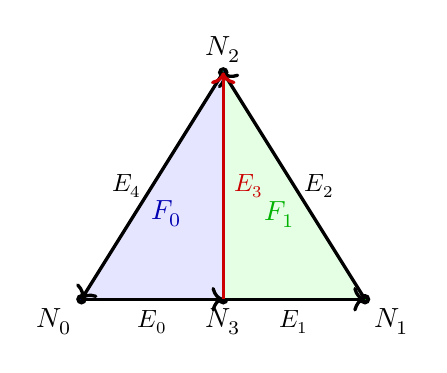
\begin{tikzpicture}[scale=1.2, dot/.style={fill, circle, inner sep=1.6pt}]
\coordinate (N0) at (0,0);
\coordinate (N1) at (3.0,0);
\coordinate (N2) at (1.5, 2.4);
\coordinate (N3) at (1.5, 0);

\fill (N0) circle (1.6pt) node[below left]  {$N_0$};
\fill (N1) circle (1.6pt) node[below right] {$N_1$};
\fill (N2) circle (1.6pt) node[above]       {$N_2$};
\fill (N3) circle (1.6pt) node[below]       {$N_3$};

\fill[blue!10, draw=blue!70!black, thin] (N0)--(N3)--(N2)--cycle;
\node[blue!70!black] at (0.9, 0.9) {$F_0$};

\fill[green!10, draw=green!70!black, thin] (N3)--(N1)--(N2)--cycle;
\node[green!70!black] at (2.1, 0.9) {$F_1$};

\draw[very thick,->] (N0)--(N3) node[midway,below] {\small $E_0$};
\draw[very thick,->] (N3)--(N1) node[midway,below] {\small $E_1$};
\draw[very thick,->] (N1)--(N2) node[midway,right] {\small $E_2$};
\draw[very thick,->] (N2)--(N0) node[midway,left] {\small $E_4$};
\draw[very thick,->,red!80!black] (N3)--(N2) node[midway,right] {\small $E_3$};
\end{tikzpicture}
\end{center}
\end{block}
\end{frame}

\begin{frame}{Example}
    \begin{block}{Coboundary Matrices \(\overline{\delta}_0,\overline{\delta}_1\)}
From the consistent boundary operators
\(\overline{\partial}_1\in\mathbb{R}^{4\times 5}\),
\(\overline{\partial}_2\in\mathbb{R}^{5\times 2}\):
\vspace{-0.3cm}
\begin{align*}
\overline{\delta}_0
&=\overline{\partial}_1^{\mathsf{T}}
=
\begin{array}{c}
\\[-0.25cm]
\scriptstyle E^0\\[-0.05cm]
\scriptstyle E^1\\[-0.05cm]
\scriptstyle E^2\\[-0.05cm]
\scriptstyle E^3\\[-0.05cm]
\scriptstyle E^4
\end{array}
\left[
\begin{array}{cccc}
\scriptstyle N^0 & \scriptstyle N^1 & \scriptstyle N^2 & \scriptstyle N^3\\ \hline
-1&  0&  0&  1\\
 0&  1&  0& -1\\
 0& -1&  1&  0\\
 0&  0&  1& -1\\
 1&  0& -1&  0
\end{array}
\right],\\[6pt]
\overline{\delta}_1
&=\overline{\partial}_2^{\mathsf{T}}
=
\begin{array}{c}
\\[-0.25cm]
\scriptstyle F^0\\[-0.05cm]
\scriptstyle F^1
\end{array}
\left[
\begin{array}{ccccc}
\scriptstyle E^0 & \scriptstyle E^1 & \scriptstyle E^2 & \scriptstyle E^3 & \scriptstyle E^4\\ \hline
 1 &  0 &  0 &  1 &  1\\
 0 &  1 &  1 & -1 &  0
\end{array}
\right].
\end{align*}
\end{block}
\end{frame}


\begin{frame}{Example}
    \begin{block}{Actions on Cochains}
Let $\sigma\in C^0M$ and $\rho\in C^1M$. Then
\vspace{-0.3cm}
\begin{align*}
(\delta_0\sigma)(E_3)&=\sigma\!\big(\partial_1E_3\big)
=\sigma(N_2-N_3)=\sigma(N_2)-\sigma(N_3),\\
(\delta_1\rho)(F_0)&=\rho\!\big(\partial_2F_0\big)
=\rho(E_0+E_3+E_4)=\rho(E_0)+\rho(E_3)+\rho(E_4),\\
(\delta_1\rho)(F_1)&=\rho\!\big(\partial_2F_1\big)
=\rho(E_1+E_2-E_3)=\rho(E_1)+\rho(E_2)-\rho(E_3).
\end{align*}
\end{block}

\begin{block}{Historical Note: Georges de Rham}
Georges de Rham (1903–1990) was a Swiss mathematician who pioneered the connection between differential forms and topology. His work led to the \textbf{de Rham theorem}, establishing the equivalence between differential and topological cohomology - the foundation of the modern de Rham map. \tiny{see next}
\end{block}
\end{frame}
%---------------------------
\begin{frame}{de Rham Map}
\vspace{-0.3cm}
\begin{block}{Definition}
Let $X$ be a smooth manifold with $\dim X=D$, and let $M$ be a CM embedded by
$\varphi:M\hookrightarrow \mathcal{P}(X)$. For $p\in\{0,\dots,D\}$, define
\[
R_p:\Omega^p(X)\to C^pM,\qquad
(R_p\omega)(c):=\int_{\varphi(c)}\omega,\quad c\in M_p,
\]
and extend by linearity to chains.
\end{block}
\vspace{-0.3cm}
\begin{block}{Example on the Interval \(X=[0,2]\)}
Nodes: $N_0,N_1,N_2$ at $x=0,1,2$.
Edges: $E_0=[0,1]$, $E_1=[1,2]$ with the natural left-to-right orientation.
\begin{center}
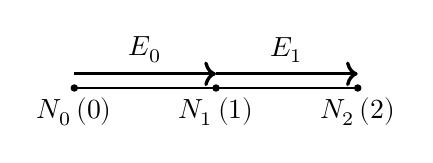
\begin{tikzpicture}[scale=0.9]
\draw[thick] (0,0)--(4,0);
\fill (0,0) circle(1.5pt) node[below] {$N_0\,(0)$};
\fill (2,0) circle(1.5pt) node[below] {$N_1\,(1)$};
\fill (4,0) circle(1.5pt) node[below] {$N_2\,(2)$};

\draw[very thick,->] (0,0.2)--(2,0.2) node[midway,above] {$E_0$};
\draw[very thick,->] (2,0.2)--(4,0.2) node[midway,above] {$E_1$};
\end{tikzpicture}
\end{center}
\vspace{-0.4cm}
\end{block}
\end{frame}

\begin{frame}{Example}
    \begin{block}{Concrete Evaluation}
For $p=0$ (functions $f\in\Omega^0(X)$):
\vspace{-0.3cm}
\begin{align*}
(R_0 f)(N_i)&=\int_{\{x_i\}} f \;=\; f(x_i),\qquad x_0=0,\ x_1=1,\ x_2=2.
\end{align*}
For $p=1$ ($\omega=g(x)\,dx\in\Omega^1(X)$):
\vspace{-0.3cm}
\begin{align*}
(R_1\omega)(E_0)=\int_{0}^{1}\!g(x)\,dx,\qquad
(R_1\omega)(E_1)=\int_{1}^{2}\!g(x)\,dx.
\end{align*}
Thus $R_0:\Omega^0\to C^0M$ samples at nodes; $R_1:\Omega^1\to C^1M$ integrates along oriented edges.
\end{block}
\end{frame}

%---------------------------
\begin{frame}{Discrete Stokes–Cartan}
\vspace{-0.2cm}
\begin{block}{Theorem (de Rham–Coboundary Commutativity)}
For $p\in\{0,\dots,D-1\}$,
\vspace{-0.3cm}
\begin{align*}
R_{p+1}\circ d_p \;=\; \delta_p\circ R_p.
\end{align*}
\end{block}

\begin{center}
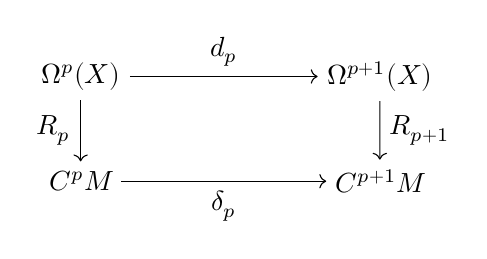
\begin{tikzpicture}[scale=0.95]
% nodes
\node (OmP) at (0,1.2) {$\Omega^p(X)$};
\node (OmP1) at (4,1.2) {$\Omega^{p+1}(X)$};
\node (Cp) at (0,-0.2) {$C^p M$};
\node (Cp1) at (4,-0.2) {$C^{p+1} M$};

% arrows
\draw[->] (OmP)  -- node[above] {$d_p$} (OmP1);
\draw[->] (OmP)  -- node[left]  {$R_p$} (Cp);
\draw[->] (Cp)   -- node[below] {$\delta_p$} (Cp1);
\draw[->] (OmP1) -- node[right] {$R_{p+1}$} (Cp1);
\end{tikzpicture}
\end{center}
\vspace{-0.3cm}
\begin{block}{Specialization (e.g.\ \(D=3\))}
For $p=0,1,2$ the same commutative diagram holds with
$\Omega^p(\mathbb{R}^3)$ and $C^pM$ (vertices, edges, faces) embedded in $X=\mathbb{R}^3$ by $\varphi$.
\end{block}
\end{frame}

%---------------------------
\begin{frame}{Discrete and Smooth Trace}
\begin{block}{Definition (Discrete Trace)}
Let $L\subseteq M$ be a submesh. The trace
\[
\operatorname{tr}_p: C^pM \longrightarrow C^pL,\qquad
(\operatorname{tr}_p\sigma)(c)\;=\;\sigma(c),\quad c\in L_p,
\]
is restriction of cochains to $L$.
\end{block}

\begin{block}{Compatibility (Smooth vs Discrete Trace)}
Let $\mathrm{tr}^{\mathrm{sm}}_p:\Omega^p(X)\to\Omega^p(\partial X)$ be the smooth trace (pullback to the boundary).
Then the de Rham maps commute with trace:
\vspace{-0.3cm}
\begin{align*}
\operatorname{tr}_p \circ R_p \;=\; R^{\,L}_p \circ \mathrm{tr}^{\mathrm{sm}}_p,
\end{align*}
where $R^{\,L}_p:\Omega^p(\partial X)\to C^pL$ is the de Rham map on the submesh $L$.
\end{block}

\end{frame}


\begin{frame}{Commutative Diagram}
    \begin{block}{}
        \begin{center}
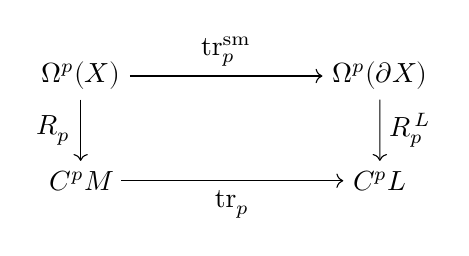
\begin{tikzpicture}[scale=0.95]
\node (Om)  at (0,1.2) {$\Omega^p(X)$};
\node (OmB) at (4,1.2) {$\Omega^p(\partial X)$};
\node (CpM) at (0,-0.2) {$C^p M$};
\node (CpL) at (4,-0.2) {$C^p L$};

\draw[->] (Om)  -- node[above] {$\mathrm{tr}^{\mathrm{sm}}_p$} (OmB);
\draw[->] (Om)  -- node[left]  {$R_p$} (CpM);
\draw[->] (CpM) -- node[below] {$\operatorname{tr}_p$} (CpL);
\draw[->] (OmB) -- node[right] {$R^{\,L}_p$} (CpL);
\end{tikzpicture}
\end{center}
    \end{block}
\end{frame}

\begin{frame}{Summary of Combinatorial Foundations}
\begin{block}{Discrete Geometry Essentials}
\begin{itemize}
\item \textbf{$p$–cells:} Basic building blocks — single points ($p{=}0$) or open $p$–balls ($p{>}0$).
\item \textbf{Regular cell complex:} A collection of cells closed under intersection and face closure,
      i.e.\ $\mathrm{cl}(a)=\bigcup_{b\subseteq a}b$.
\item \textbf{Combinatorial mesh:} A partially ordered set $(M,\preccurlyeq)$
      that can be embedded into a smooth manifold $X$ such that its image forms a regular cell complex.
\item \textbf{Polytopes:} Meshes with one top $D$–cell — segments ($1$D), polygons ($2$D),
      cubes/tetrahedra ($3$D), etc.
\item \textbf{Diamond property:} For $a\!\in\!M_{p+2}, c\!\in\!M_p$ with $c\!\prec\!a$, there exist exactly two
      $(p{+}1)$–cells $b'$ and $b''$ such that
      $c\!\prec\!b',b''\!\prec\!a$.
\end{itemize}
\end{block}
\end{frame}


\begin{frame}{Summary of Chain Complex Structure}
\begin{block}{Orientation and Boundary Operators}
\begin{itemize}
\item \textbf{Relative orientation:} $\epsilon(a,b)\in\{\pm1\}$ defines the signed incidence between adjacent cells
      satisfying $\epsilon(a,b')\epsilon(b',c)=-\epsilon(a,b'')\epsilon(b'',c)$.
\item \textbf{Chains:} $C_pM = \mathrm{Free}_{\mathbb{R}}(M_p)$ - linear combinations of oriented $p$–cells.
\item \textbf{Boundary operator:}
      \vspace{-0.3cm}
      \begin{align*}
      \partial_p(a)=\sum_{b\prec a}\epsilon(a,b)\,b, \qquad \partial_{p+1}\circ\partial_{p+2}=0.
      \end{align*}
\item \textbf{Example (triangular cell with diagonal):} Explicit $\partial_1$, $\partial_2$ matrices verified
      $\overline{\partial}_1\overline{\partial}_2=0$.
\end{itemize}
\end{block}
\end{frame}

\begin{frame}{Summary of Discrete Differential}
\begin{block}{Dual Spaces and Operators}
\begin{itemize}
\item \textbf{Cochains:} $C^pM = (C_pM)^*$ - linear duals of $p$–chains.
\item \textbf{Coboundary operator:} $\delta_p = \partial_{p+1}^T$ defines the discrete analogue of the exterior derivative,
      satisfying $\delta_{p+1}\circ\delta_p=0$.
\item \textbf{Example:} Explicit matrices $\overline{\delta}_0,\overline{\delta}_1$ act on cochains:
      \vspace{-0.3cm}
      \begin{align*}
      (\delta_0\sigma)(E_i)=\sigma(\partial_1E_i),\quad
      (\delta_1\rho)(F_j)=\rho(\partial_2F_j).
      \end{align*}
\item \textbf{de Rham map:} $R_p:\Omega^p(X)\!\to\!C^pM$ with
      \vspace{-0.3cm}
      \begin{align*}
      R_{p+1}\circ d = \delta_p\circ R_p,
      \end{align*}
      establishing equivalence between smooth and discrete calculus.
\item \textbf{Trace consistency:} $\operatorname{tr}_p^{\text{disc}}\!\circ R_p^{M}
      = R_p^{L}\!\circ \operatorname{tr}_p^{\text{smooth}}$.
\end{itemize}
\end{block}
\end{frame}

\begin{frame}{Thanks}
  \cmcendframe
\end{frame}

\end{document}
